
\subsection{Trigonometri}

\subsubsection{Sinus Relationerne}
\begin{minipage}{0.4\textwidth}
    \[
    \frac{a}{\sin(A)} = \frac{b}{\sin(B)} = \frac{c}{\sin(C)}
    \]
\end{minipage}
\hfill
\begin{minipage}{0.4\textwidth}
    \[
    \frac{\sin(A)}{a} = \frac{\sin(B)}{b} = \frac{\sin(C)}{c}
    \]
\end{minipage}

\begin{figure}[H]
    \centering
    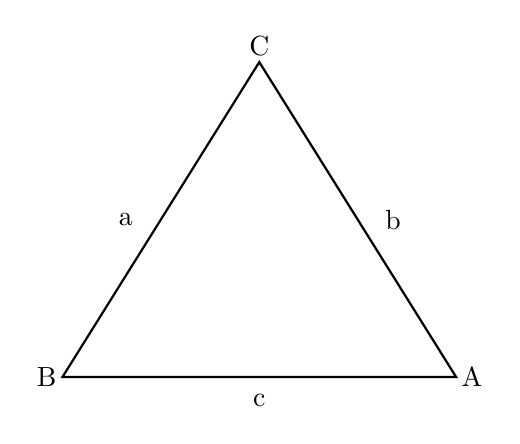
\begin{tikzpicture}[scale=1]
        \draw[thick] (0,0) -- (5,0) -- (2.5,4) -- cycle;
        
        % Side labels
        \node at (2.5,-0.3) {c};
        \node at (4.2,2) {b};
        \node at (0.8,2) {a};

        % Point labels
        \node at (-0.2,0) {B};
        \node at (5.2,0) {A};
        \node at (2.5,4.2) {C};

    \end{tikzpicture}
\end{figure}

\subsubsection{Cosinus Relationerne}
\

\begin{minipage}{0.5\textwidth}
    \centering
    \textbf{2 sider og mellemliggende vinkel}
    \[
        a^2 = b^2 + c^2 - 2\cdot b\cdot c\cdot \cos(A)
    \]
    \[
        b^2 = a^2 + c^2 - 2\cdot a\cdot c\cdot \cos(B)
    \]
    \[
        c^2 = a^2 + b^2 - 2\cdot a\cdot b\cdot \cos(C)
    \]
\end{minipage}
\hfill
\begin{minipage}{0.3\textwidth}
    \centering
    \textbf{3 sider}
    \[
        cos(A) = \frac{b^2 + c^2 - a^2}{2\cdot b\cdot c}
    \]
    \[
        cos(B) = \frac{a^2 + c^2 - b^2}{2\cdot a\cdot c}
    \]
    \[
        cos(C) = \frac{a^2 + b^2 - c^2}{2\cdot a\cdot b}
    \]
\end{minipage}
